La gerarchia vuole modellare degli oggetti che comprendono tutti i file audio-visivi ed è così composta: una classe base astratta denominata \texttt{AudioVisual} e tre classi derivate \texttt{TvSerie}, \texttt{Movie}, \texttt{Documentary} che implementano i metodi puri della classe base. 

\begin{center}
    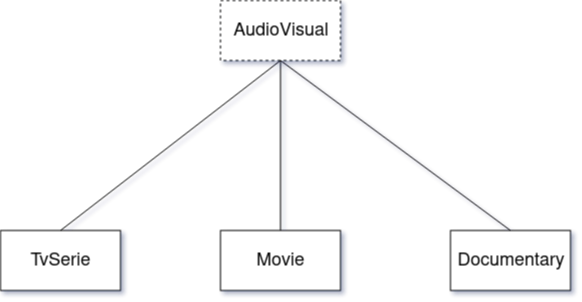
\includegraphics[width=0.6\textwidth]{gerarchia}
\end{center}

\paragraph{AudioVisual}
La classe base della gerarchia fornisce le informazioni di base comuni a tutti i file di tipo audio-visivo, ossia il \textit{titolo} del file, l'\textit{immagine} di copertina, la \textit{descrizione} della trama, la \textit{data} di rilascio espressa in anni, la \textit{durata} in minuti, il nome del \textit{regista}, se il file appartiene ai \textit{preferiti} dell'utente, se l'audio è \textit{compresso} o meno, la \textit{risoluzione} dell'immagine, i \textit{frame per secondo}.

\paragraph{TvSerie}
TvSerie è una classe derivata concreta rappresenta i file riguardanti le serie tv, infatti aggiunge i campi dati riguardanti il numero di \textit{episodi} della serie, il numero di \textit{stagioni}, se la serie è \textit{terminata}, il \textit{rating}, il \textit{genere}, il \textit{cast} formato dai personaggi.

\paragraph{Documentary}
Documentary è una classe derivata concreta che rappresenta i file di tipo documentario, in cui si ha un \textit{topic} che spazia dall'argomento scientifico, a quello storico o biografico e un campo dati riservato al \textit{narratore}.

\paragraph{Movie}
Movie è anch'essa una classe derivata concreta che vuole rappresentare i file di tipo film; aggiunge i campi dati riguardanti il \textit{cast}, il \textit{rating} ed il \textit{genere}. 

La gerarchia attuale è stata pensata per essere estensibile in futuro, sia in orizzontale, per esempio implementando una classe riguardante i video di YouTube, che in vertiale, per esempio derivando da \texttt{TvSerie} una classe che rappresenti le telenovelas. \newline
Inoltre non fa uso di dati o classi riguardanti il framework QT, per cui è indipendente da esso.

\paragraph{DeepPtr}
Il progetto fa uso anche di un template di classe \texttt{DeepPtr<T>} di puntatori polimorfi al tipo T che implementano la gestione automatica della memoria cosidetta profonda. È quindi necessario che ogni classe concreta della gerarchia implementi il metodo relativo alla clonazione e anche la distruzione polimorfa.

\paragraph{Polimorfismo}
%metodi virtuali puri utilizzati all'interno, quali clone utile per lo smart pointer implementato. 



\begin{comment}
%4k, 144p, 240, 480, 360, 720
%4k/2160p, FullHD/1080p, HD/720p, SD/480p, LD/240p

I metodi sono:
\begin{itemize}
    \item Clone : metodo usato da deepptr per la costruzione di copia profonda
    \item Operatore di uguaglianza e disuguaglianza
    \item isFavorite : metodo usato per sapere se un "AudioVisual" è tra i preferiti dell'utente
    \item getTotalRunningTime : metodo che restituisce il tempo totale di un AudioVisual o sotto tipo
    \item getType : restituisce il tipo dell'oggetto d'invocazione ("tipo")
    \item getQuality : Audio + Video % se definisco dei range diversi per ogni sottotipo allora questo metodo è virtuale puro
    \item get : genere + rating 
\end{itemize}

\paragraph{User}
I campi dati sono:
\begin{itemize}
    \item Nickname
    \item TotalTime
\end{itemize}
I metodi sono:
\begin{itemize}
    \item getTotalTime : somma di tutti i RunningTime degli AudioVisual appartenenti alla lista
\end{itemize}

\end{comment}